% !TEX root = ../thesis.tex
% !TeX spellcheck = en_US

In this chapter, basic concepts are described, which are relevant for this thesis.
Primarily, this includes geodata, routing algorithms as well as agent-based simulations.
The section about geodata gives a broad overview of coordinate systems, file formats, standards and OpenStreetMap, which is the source of geodata in this thesis.
Geodata in general can be used to find shortest paths between two locations using routing algorithms.
Two main strategies exist to find such paths, graph-based and geometric routing, and both will be covered in this chapter.
Agent-based simulations play an important role in pedestrian simulations and often use these routing algorithms for the agent's movements.
Hence, the topic of agents and simulations will be covered as well.

\section{Geospatial data}

	According to the ISO standard 19109:2015\cite{iso-19109}, the term \term{geospatial data} refers to \enquote{data with implicit or explicit reference to a location relative to the Earth}.
	In other words, data with any kind of address, coordinate or other location reference belongs to the class of \term{geospatial data}, or \term{geodata} for short.
	
	Examples are customer information (address information of each customer), meteorological data (measured temperature and humidity with a coordinate and altitude) and, primarily used in this thesis, road and path data suitable for routing.
	Since addresses are not globally standardized, describe only a vague location and usually belong to a whole area, they are of less importance for this thesis.
	Geodata with an additional time dimension is also categorized as \term{spatiotemporal data}\cite{iso-19108} and even though the time dimension is relevant to many real-world use cases, this type of data is of less importance for this thesis as well.
	The term \emph{geodata} in this thesis refers to data structures as described below in \Cref{subsec:data-structures}.
	
	Besides the mentioned explicit references to locations, such as coordinates, implicit location references can be encoded within metadata of datasets as well.
	This is for example the case with the image-based GeoTIFF format, which stores the geographic extent of the image in the metadata of a normal TIFF image file\cite{ogc-geotiff}.
	The exact coordinate of a data point (in this case a pixel in the TIFF image), must then be calculated using this metadata.

	\subsection{Coordinate reference systems and projections}
	
		Coordinates are used to specify exact locations on Earth.
		However, the Earth is not a perfect sphere but rather an ellipsoid.
		But even this ellipsoid is not smooth and has slightly different radii in different regions.
		Furthermore, most regions on Earth move due to continental drift and therefore constantly change their positions and distances relative to each other.
		Even though the continental plates move slowly, this effect adds up to a significant distance rendering very accurate measurements potentially unusable over time\cite[7]{ordenance-survey-booklet}.
		These properties of Earth's surface make it necessary to have a variety of different reference systems and projections for spatial data covering different parts of the planet.
		
		A \term{coordinate reference system} (CRS) defines the combination of a coordinate system and an approximation of the surface of the Earth.
		The \term{coordinate system} defines the extent, meaning the spatial boundaries, and unit of coordinates.
		Types of coordinate systems are for example Cartesian (coordinates in meters or foot) and ellipsoidal (coordinates in degrees)\cite[11-13]{ordenance-survey-booklet}.
		The \term{horizontal datum} (also \term{Terrestrial Reference System} or \term{geodetic datum}) defines the origin and orientation of the coordinate system and is therefore a mapping from a numeric coordinate to a real location on Earth based on a specific ellipsoid.
		
		\term[ellipsoid]{Ellipsoids} are deformed spheres, which describe either the whole Earth or a part of it, e.g. a single continent or country, as accurately as possible.
		Depending on this ellipsoid, the horizontal datum either defines a global or local reference system.
		The latter is more accurate in certain places while a global system is designed to find good approximations for every location on Earth.
		Cartesian coordinate systems with two dimensions only work on flat surfaces, therefore a \term*[map projection]{projection} is required to turn each spherical location on the ellipsoid into a two-dimensional planar location in the coordinate system\cite[17]{ordenance-survey-booklet}.
		
		Analogous to the horizontal datum, a \term{vertical datum} can be used to define the height of data\cite{ordenance-survey-booklet}.
		This is done by defining a so-called \term{geoid}, which defined the level of zero height.
		Such a geoid can be modeled using another ellipsoidal sphere but that would result in very inaccurate data.
		Instead, local reference levels for height data are used, such as the Ordnance Datum Newlyn (\term*{ODN}) for Britain or Normalhöhennull (\term*{NHN}) for Germany.
		Since it is often based on the water level of oceans, the level of zero height on landmasses is extrapolated based on the gravitational field of the Earth.
		
		For visualization purposes, a \term{map projection} might be needed to translate coordinates from the CRS of the data into the coordinate system used of the map.
		The map can be two-dimensional but digital maps can also be rendered on a three-dimensional sphere.
		Since the projections of the data and map can differ, transformations between the projections are needed.
		
		For better communication, the European Petroleum Survey Group (\term*{EPSG}) created a database with definitions for coordinate reference systems and transformations\cite{epsg}.
		Each entry in this database has an ID with the prefix \enquote{EPSG:} followed by a numeric code, for example EPSG:4326 refers to the global and widely used World Geodetic System 1984 (WGS 84), a global ellipsoidal horizontal datum used for example in GPS.
		
	\subsection{Data structures}
	\label{subsec:data-structures}
	
		Spatial data can be stored in a variety of data structures.
		Some of these are used in many frameworks, libraries and formats, but some are vendor specific.
		An overview of common data structures in spatial data is given in this section.
		
		The \term{Simple Feature Access} (\term*{SFA}) standard by the Open Geospatial Consortium (\term*{OGC}) defines numerous geometry types\cite{ogc-sfa}, however, not all of them are implemented in all data formats and most of them are not relevant for this thesis.
		The GeoJSON file format (described in more detail in \Cref{subsubsec:geojson}) implements the most important geometries and data structures of the SFA standard\cite{ietf-geojson}.
		Therefore, an overview of these geometry types as well as an introduction to the concept of features is given in this section.
		
		\subsubsection{Geometries}
		
			A \term{geometry} just represents geometric coordinates and their relation to each other.
			Common types of geometries are:
			\begin{description}
				\item[Point] Simple geometry type with only one coordinate.
				\item[LineString] An ordered list of multiple coordinates building a line with a certain direction.
				\item[Polygon] An ordered list of coordinates of which the first and last coordinates are equal and thus form an area. A polygon might consist of additional polygons inside of it forming holes. Polygons inside such holes form islands, which in turn can have holes again.
				\item[Multi-Geometries] Grouping geometries of the same type together forms multi-geometries, such as \texttt{MultiPoint}, \texttt{MultiLineString} and \texttt{MultiPolygon}. They can be used to share properties of the contained geometries.
			\end{description}
		
		\subsubsection{Features}
		
			According to the OGC, a \term{feature} is an \enquote{abstraction of real world phenomena}\cite{ogc-sfa}, for example a tree, road or lake.
			It therefore consists of a geometry, describing \textit{where} the feature is, and certain attributes (also called \enquote{properties} or \enquote{tags}), describing \textit{what} the feature represents.
			In the case of GeoJSON, these attributes consist of any number of key-value pairs that can contain arbitrary entries.
			Some other file formats might have technical restrictions regarding possible attributes (e.g. the number of bytes per value) while others try to standardize the allowed keys and values.
		
		\subsubsection{Standardization}
		
			Standards exist to keep a data source consistent but to also allow interoperability between systems.
			Common standards were defined by organizations like the OGC as well as companies or government agencies.
			
			A widely used proprietary standard established by the company Esri Inc. is the Shapefile file format, which will be covered in \Cref{subsubsec:other-formats}.
			
			One example for a governmental standard is the INSPIRE standard.
			It was established based on an initiative of the European Commission and defines fixed attributes with keys and values as well as specifications for metadata.
			This standard works on a high level of detail with numerous separate specifications for different types of features, for example there exists a single specification just for protected sites, such as natural reserves\cite[31]{inspire-protected-sites}.
		
			A standardization strategy based on democratic votes is used by \term*{OpenStreetMap}.
			This procedure takes place in the project's Wiki, where voting takes place and keys with their according values are defined.
			However, arbitrary tags (key-value pairs) are still explicitly allowed to ensure a high degree of flexibility\cite{osm-wiki-proposal-process}.
			Details on OSM are given in \Cref{subsec:osm}.
			
	\subsection{File formats}
	\label{subsec:file-formats}
	
		Spatial data can be stored in a variety of different file formats with different properties and use cases.
		Both proprietary and open standards exist and are used frequently in scientific and real-world applications.
		The \term[OGC]{Open Geospatial Consortium} (OGC) publishes open standard definitions and schemas for some of these open file formats.
		This section gives an overview of some popular formats.
		
		\subsubsection{GeoJSON}
		\label{subsubsec:geojson}
		
			Another open but not OGC-standardized format is \term{GeoJSON}, which is the most important format for this thesis as all used datasets were in this file format.
			As the name suggests, a GeoJSON file follows the JSON specification as defined in \href{https://datatracker.ietf.org/doc/html/rfc7946}{RFC7946}\cite{ietf-geojson}.
			The file can either contain a collection of features or geometries.
			Both collections are represented by a designated type, namely \texttt{GeometryCollection} and \texttt{FeatureCollection}.
			A \texttt{GeometryCollection} is itself one possible geometry type.
			Each feature in a \texttt{FeatureCollection} consists of a geometry and, in contract to elements in a \texttt{GeometryCollection}, attributes adding additional information to the feature.
			The number of geometries per feature as well as the length, number and character choice of attributes is not restricted.
			The CRS is fixed and has been set to WGS 84.
			
		\subsubsection{GeoTIFF}
		
			All formats mentioned so far store vector data, but raster data can be georeferenced as well.
			One image-based format to store such raster data is the OGC-standardized \term{GeoTIFF} format\cite{ogc-geotiff}, which is an TIFF formatted image with spatial metadata such as the CRS and a mapping of pixel to coordinates.
			Typical use cases for such images are aerial or satellite imagery and \term*[digital elevation model]{digital elevation models} (\term*{DEM}).
			However, other use-cases are thinkable, such as field-based routing algorithms as mentioned in \Cref{subsec:field-based-routing} using raster data to store the vector fields.
		
		\subsubsection{Other formats}
		\label{subsubsec:other-formats}
		
			There are many more formats for numerous use cases ranging from simple unstandardized to complex, feature rich and fully standardized formats.
			
			A \emph{comma-separated value} (\term*{CSV}) file can also serve as a spatial file format where certain columns contain geographical information.
			The simplicity of this format is its biggest advantage and it is used as transportation format for many public datasets.
			One example is the publicly available timetable data of the HVV (public transport network in Hamburg, Germany)\cite{hvv-fahrplandaten}.
			
			The \term{Well-known Text} (\term*{WKT}) format is a simple, text-based format specified by the OGC\cite[51]{ogc-sfa}.
			One popular use case is communication with databases.
			
			More complex formats are \term{SpatiaLite} and \term{GeoPackage}.
			SpatiaLite specifies an extension to file-based SQLite database engine and offers additional geodata specific functionality\cite{spatialite-website}.
			The GeoPackage format is very similar to SpataLite as it is based on an SQLite database as well, but it diverged from the SpatiaLite format, for example by using a different WKB encoding\cite{geopackage-faq}.
			
			The \term[kml]{Keyhole Markup Language} (KML) is a XML-based format with the ability to contain much more data than just spatial features, such as the lifetime of data or camera positions used for visualization purposes \cite{ogc-kml-2.2}.
			
			Another widely used format is the proprietary \term[shapefile]{Esri Shapefile} format, which was developed in the 1990s by the company Esri \cite{esri-shapefile-file-ext-spec} and is often used in Esri products like the ArcGIS platform.
			One shapefile actually consists of multiple separate files containing projection information, indices or attributes.
			Dispite its popularity, the shapefile format contains numerous technical limitations, such as the restriction of one geometry type per shapefile, a limit of ten characters per attribute name, a limit of 254 characters on attribute values or the overall maximum number of 255 attribute per feature.
			
	\subsection{OGC web services}
	
		Besides file-based formats, web-based standards exist as well.
		The OGC standardized some APIs for web-based services.
		Popular standards are the \term{Web Map Service} (\term*{WMS}), \term{Web Map Tile Service} (\term*{WMTS}) and \term{Web Feature Service} (\term*{WFS}).
		These services are only used to interact with the raw data but do not offer higher-level functionalities such as routing.
	
	\subsection{GIS}
	
		A file format alone, as described in \Cref{subsec:file-formats}, is only useful when it comes to storing or transferring data ensuring interoperability.
		Processing the data is part of applications referred to as \term[geographic information system]{geographic information systems} (\term*{GIS}).
		
		The term GIS is very broad and describes nearly all systems working with spatial data.
		This includes databases like Postgres with the PostGIS extension, processing tools like GDAL, libraries like the Net Topology Suite, servers like GeoServer and desktop applications like ArcMap or QGIS.
		Such desktop application often combine multiple functionalities to visualize, analyze or otherwise process the data.
	
	\subsection{OpenStreetMap}
	\label{subsec:osm}
	
		\term{OpenStreetMap} (\term*{OSM}) is a geospatial database that is maintained by a global community and licensed under the \term{Open Data Commons Open Database License} (\term*{ODbL})\cite{osm-wiki-about}.
		It can therefore be used, changed and redistributed as long as a proper attribution is given and results stay under the ODbL\cite{odbl-summary}.
		All spatial data used in this thesis is data from the OSM database.
		In 2006, two years after the OSM project started, the OpenStreetMap Foundation was established to perform fund-raising, maintain the servers and also act as a legal entity for the project.
		People contributing to OSM are called \textit{mappers} or simply \textit{contributors} and most of them are volunteers, often mapping their local vicinity or concentrating on specific topics.
		However, a rising number of companies with payed mappers contribute as well, adding data beneficial for their business model\cite{osm-corporate-mappers}.
		
		\subsubsection{Data model}
		
			The model of OSM is much simpler compared to many of the \hyperref[subsec:file-formats]{aforementioned} data formats.
			There are three main data types in OSM: \term{node}, \term{way} and \term[relation]{relations}\cite{osm-wiki-data-model}.
			
			Nodes and ways are analogous to \texttt{Point} and \texttt{LineString} from the OGC \term*{Simple Feature Access} (\term*{SFA}) specification described in \Cref{subsec:data-structures}.
			Areas also exist but they are modeled as closed ways and therefore do not form a new type of geometry.
			A way is closed when the first and last coordinates are identical and certain area compatible attributes exist.
			
			Relations form multi-geometries, so they are analogous to \texttt{MultiPoint}, \texttt{MultiLineString} and \texttt{MultiPolygon} of the SFA specification.
			Typical use cases are multipolygons, turn restrictions and bus routes.
			Each element in a relation can have the optional attribute \texttt{role} specifying \enquote{the function of a member in the relation}\cite{osm-wiki-relation}.
			Example values for this role are \texttt{outer} and \texttt{inner} for rings in a multipolygon, \texttt{from}, \texttt{via} and \texttt{to} for turn restrictions or \texttt{stop} and \texttt{platform} in a bus route.
			
		\subsubsection{Attributes}
		\label{subsubsec:osm-attributes}
			
			Attributes are called \term[tag]{tags} and are simple unrestricted key-value pairs.
			Most tags describe the properties of the feature.
			For example a node may have tags making it a restaurant with additional tags for the name, address and opening hours.
			
			Some tags, like \texttt{area=[yes|no]} or the \texttt{type} key used for relations, influence the type of geometry.
			A closed way with \texttt{area=no} does, in fact, \textit{not} represent a polygon, but a closed line.
			This not only affects visualizations but may also need to be considered in other processing and analysis tasks.
			
			Other tags add metadata to objects, for example the last time the feature was surveyed, the source of the data or internal notes to other mappers.
			
			Standardization of tags takes place in the project's wiki via a special proposal process.
			To ensure flexibility, it is explicitly allowed to use new, reasonable and unstandardized tags\cite{osm-wiki-proposal-process}, which are de-facto accepted if they are commonly used.
			The community tries to organize and professionalize the development of new tags using the proposal process.
			Not only can a proposed tagging scheme be accepted or rejected by a democratic vote, a mandatory public discussion of a minimum duration needs to take place earlier.
			Due to the vast amount of contributors, different opinions, use cases, editors and knowledge about the tagging schemes, multiple competing schemes might evolve (for example \texttt{phone=*} and \texttt{contact:phone=*}).
			Tagging schemes change over time and some may become deprecated or are officially abandoned via a proposal, leading to outdated tags on objects.
			
		\subsubsection{Contributions to OSM}
		
			Uploads to OSM always happen in so-called \term[changeset]{changesets} combining multiple changes on the map\cite{osm-wiki-changeset}, they can therefore be seen as a kind of transaction.
			Like features, each changeset itself can have tags adding metadata to the change.
			The \texttt{created\_by}, \texttt{comment} and \texttt{source} tags are the most common ones but more details can be added depending on the editor being used.
			
			% TODO kürzen/weglassen?
			Because some mappers also perform manual quality assurance by reviews, each changeset should fulfill certain quality criteria.
			The simplest one is a good changeset comment containing information about \textit{what} changed and \textit{why} the change was necessary.
			For legal reasons, specifying the source is very important since the ODbL is not necessarily compatible with licenses of other data sources.
			Ideally, a changeset should be coherent, which means that it should focus on one thematic aspect in one local area.
			Too large and crowded changesets are difficult to maintain and therefore might get reverted.
			
		\subsubsection{Data contained in OSM}
		
			Since OSM has no focus on specific topics and due to the flexible tagging scheme \hyperref[subsubsec:osm-attributes]{mentioned above}, nearly anything can be added to OSM.
			However, there are some types of features that are very common according to \href{https://taginfo.openstreetmap.org/keys}{taginfo.openstreetmap.org}, a service providing daily updated statistics on keys and values in OSM\cite{taginfo-keys}.
			According to these statistics, the most common objects are buildings with over 542 million occurrences.
			In fact, 6\% of all objects and nearly 60\% of all ways are buildings.
			Highways (mainly roads and streets but also paths, bridleways, railways and more) are the second common type of features with over 219 million ways (23\% of all ways).
			Addresses are also very common, about 32\% of all nodes and 7\% of all ways (mainly building) have a house number.
			Other often added area features are forests and lakes as well as line features like barriers and waterways.
			
		\subsubsection{Data \textit{not} contained in OSM}
		\label{subsubsec:data-not-in-osm}
		
			Even though the tagging scheme can be extended arbitrarily, some data will probably not be added to OSM.
			This can have multiple reasons.
			
			First, some data is too detailed and therefore people will not invest the time necessary to create or maintain that data.
			For example a tree can have tags specifying its genus, species, taxon, Wikipedia and Wikidata references to each of these, leaf type, leaf cycle, protection, circumference, height, an image and even more. Some, especially older, protected or locally important trees, do have some of these tags, but the vast majority has none of these tags apart from the necessary \texttt{natural=tree}.
			
			Second, OSM follows some strategies on what and what not to add.
			One important strategy is the verifiability of objects on the ground.
			Anyone visiting a certain place should be able to find the data from OSM and therefore verify its existence and correctness.
			
			Third, temporary data should not be added since OSM is not a real-time database.
			However, there's not a strict definition when a feature is temporary and when it is (potentially) permanent.
			
			And fourth, data under an incompatible license will not be added.
			This also includes data from many public authorities and nearly all companies.
			
			Unfortunately, data relevant to routing is often added to ways representing roads and paths, but not to areas.
			This includes primarily accessibility and surface information.
			However, the latter can potentially be inferred or approximated from other tags on a polygon, for example \texttt{surface=grass} can be inferred from \texttt{natural=grassland} and \texttt{access=yes} from \texttt{place=square}.
			However, automatic inference of tags always leads to a certain amount of errors.
			
			Private areas are often not part of OSM or contain only very little details.
			This is mainly due to the second reason from above, that private areas can often not be entered and are therefore unverifiable for unauthorized mappers, and is also based on a general awareness of privacy towards companies and residents.
			
		\subsubsection{Data used in this thesis}
		
			This thesis uses OSM data for routing purposes.
			Other sources of spatial data exist but are non-free (in terms of a price and the license of the data), fragmented over multiple sources (files, servers, APIs) or not as detailed as OSM.
			
			One example of such a fragmented source is provided by the state office for geoinformation and surveying (Landesbetrieb für Geoinformationen und Vermesseung -- LGV) in Hamburg, Germany.
			The road network and building data can be downloaded via the official website \href{https://geoportal-hamburg.de}{geoportal-hamburg.de} but are contained in two different datasets (called \enquote{HH-SIB} and \enquote{ALKIS}).
			In addition to the fragmentation, official data is not necessarily made to be used in routing algorithms.
			In fact, the road network of the \enquote{HH-SIB} dataset contains numerous line segments representing ways and roads, which are not connected to the general road network.
			The \enquote{ALKIS} dataset also contains road data, but only the area a road occupies, which cannot be used in common graph-based routing algorithms.
			OpenStreetMap, however, offers free access to numerous usable features in one single dataset.
			
			Since geometric routing is the major topic, not only the road network is used, but also certain features of OSM, which represent obstacles to navigate around.
			The following features are considered as obstacles:
			\begin{itemize}
				\item \textbf{Barriers}: The \texttt{barrier}-tags not only describe non-passable barriers but also passable structures like gates. Thus, only specific barriers (mainly fences and walls) are considered.
				\item \textbf{Buildings}: The \texttt{building} tag as it represents buildings. However, some values, such as \texttt{building=roof}, \texttt{=no} and \texttt{=demolished}, are considered passable.
				\item \textbf{Natural areas}: Areas with the \texttt{natural}-key describe areas filled with a specific form of vegetation as well as water areas. All natural areas, which are not representing grass covered land, are considered impassable.
				\item \textbf{Railway}: Any type of railway infrastructure, especially tracks.
				\item \textbf{Waterways}: This includes any type of waterway, such as rivers, streams, canals, ditches or drains.
			\end{itemize}
			The exact choice on the passable and impassable features is debatable and depends on the domain of the simulation.
			For example, train tracks might be passable in an evacuation scenario.
			
			The road network is also used, which is done by importing all features with a \texttt{highway} key.
			Filtering out irrelevant features is not done as these features have either no effect, which is for example the case for \texttt{highway=street\_lamp} for street lamps on unconnected point geometries, or contain useful information for routing, for example \texttt{highway=stop} for stop signs.

\section{Graph-based routing}
\label{sec:graph-routing}

	\subsection{Theoretic considerations}
	\label{subsec:routing-theoretic-considerations}	
	
		Graph-based routing takes place on a graph $G=(V, E)$ with $V$ being the set of vertices and $E \subseteq V \times V$ being the set of edges connecting the vertices.
		Routing is the process of finding a path from a source $s \in V$ to a destination (or target) $t \in V$ of minimal weight using a weight function $w: E \rightarrow \mathbb{R}$.
		A path $p=\left\langle v_0, v_1, \dots v_n \right\rangle$ is an ordered list of connected vertices $v_0, v_1, \dots, v_n \in V$, which means for two consecutive vertices $v_i$ and $v_{i+1}$, $(v_i, v_{i+1}) \in E$ must hold.
		
		Often, the shortest path should be determined, thus the weight function is used to calculate the length of an edge, which is not necessarily bound to the geographic length of the edge.
		Even though the following sections refer to shortest paths, determining \enquote{optimal} (or minimal) paths is the general case.
		Thus, routing is a minimization problem, trying to find a path $p$ with the minimum sum $w(p) = \sum_i{w(v_i, v_{i+1})}$\cite[645]{cormen-introduction-to-alg}.
		
		In theoretic computer science, the fundamental problem behind routing algorithms is called the \term{shortest paths problem}, which exists in several variants\cite[644]{cormen-introduction-to-alg}.
		
		\subsubsection{\term*[single-source shortest paths]{Single-source shortest paths}}
		\label{subsubsec:single-source-shortest-path}
		
			One source vertex is given and the shortest paths to all other vertices should be determined.
			Algorithms that solve this problem are for example the Dijkstra algorithm, described in detail in \Cref{subsubsec:dijkstra}, or the Bellman-Ford algorithm, which can additionally handle negative edge weights\cite[651]{cormen-introduction-to-alg}.
		
		\subsubsection{\term*[single-destination shortest paths]{Single-destination shortest paths}}
		
			This is the opposite to the above problem.
			All shortest paths to a specific vertex from any other vertex should be found.
			However, no new algorithms are needed to solve this problem.
			Instead, the direction of each edge can be reversed, turning this problem into the single-source problem.
		
		\subsubsection{\term*[single-pair shortest paths]{Single-pair shortest paths}}
		
			The shortest path from one specific source to one specific destination vertex should be determined.
			Even though there are specialized algorithms for this problem like TRANSIT (described in \Cref{subsubsec:other-speedup-methods}), more general approaches solving the single-source problem, such as Dijkstra or algorithms based on it, are used more often.
			% TODO source on that
		
		\subsubsection{\term*[all-pair shortest paths]{All-pair shortest paths}}
		\label{subsubsec:all-pair-shortest-path}
		
			This problem is similar to the single-source problem but every vertex is a source vertex.
			A naive approach would therefore be to use an algorithm solving the single-source problem on each vertex, but there are faster ways to solve this, such as the Floyd-Warshall and Johnson's algorithm\cite[693,700]{cormen-introduction-to-alg} as well as PHAST\cite{bast-transportation-networks} with a complexity of $\Theta(|V|^2)$.
		
	\subsection{Routing engines and shortest path algorithms}
	\label{subsec:routing-engines}
		
		A \term{routing engine} is a software built to find an optimal route between a source and destination location.
		The optimality of this route is determined by a routing profile, which is a weighting function assigning a weight to each edge in the input graph.
		Routing engines might perform other operations as well, such as map matching or calculation of isochrones, which are a way to visualize the reachability of a region\cite{allen-isochrones}.
		Each isochrone is an area reachable from a given source location within the same amount of time, which is determined using routing.
		
		To find desirable paths, the weight function $w$ mentioned in \Cref{subsec:routing-theoretic-considerations} needs to be carefully chosen based on the domain of the application, vehicle type, personal preferences and other influencing factors.
		Applications in our everyday life bundle these aspects into a \term{routing profile}, which maps attributes from the input data to a certain weight.
		The input data might consist of multiple sources like a road network, a digital elevation model or additional traffic information.
		Weight functions predict the expected speed on an edge\cite{graphhopper-profile-bike-speeds}, use the length of an edge\cite{graphhopper-profile-shortest} as weight or determine the weight based on existing attributes\cite{graphhopper-profile-short-fastest}.
		
		The open source software Graphhopper is one example of a routing engine and comes with predefined profiles for different modalities and situations.
		For example the \texttt{car\_delivery} profile is made for delivery services and therefore allows routing via private roads\cite{graphhopper-routing-profiles}.
		
		To enhance performance, speedup methods were developed allowing routing queries of continental or even global sizes to be answered quickly.
		Some popular methods are \term{contraction hierarchies} or the use of \term[landmark]{landmarks}, \term[transit node]{transit nodes} and \term[hub label]{hub labels}.
		Even though there are several more approaches to increase performance, the mentioned techniques will be described with more details in \Cref{subsec:speedup-methods}.
		
		\subsubsection{Dijkstra}
		\label{subsubsec:dijkstra}
		
			Dijkstra's algorithm, often just called \term{Dijkstra}, is originated in the 1950s and can be used to solve the \term*{single-source shortest paths} problem.
			When no destination vertex is given, this algorithm creates a spanning tree rooted in the source vertex $s$ containing solely shortest paths to all other vertices.
			Despite its age, Dijkstra's algorithm and optimized versions of it are frequently used in science and real-world applications.
			\Cref{alg:dijkstra} presents an enhanced version using a priority queue for the vertices\cite[658]{cormen-introduction-to-alg}.
			
			\begin{algorithm}[h]
				\begin{algorithmic}[1]
					\ForAll{vertices $v \in V$}
						\State Set shortest path distance $v.d = \infty$ and predecessor vertex $v.\pi = undefined$
					\EndFor
					\State Insert all vertices by distance into min-queue $Q$
					\State $S = \emptyset$
					\While{$Q \neq \emptyset$}
						\State Get closest vertex: $u = Q.min$
						\ForAll{adjacent vertices $v$ of $u$}
							\State Add $u$ to $S$
							\If{the path to $v$ via $u$ is shorter than $v.d$, so if $u.d + d(u, v) < v.d$}
								\State Set $v.d = u.d + d(u, v)$ and $v.\pi = u$
							\EndIf
						\EndFor \label{alg:dijkstra:end-inner-loop}
					\EndWhile
				\end{algorithmic}
				\caption{Pseudocode of an slightly optimized version of Dijkstra's algorithm.}
				\label{alg:dijkstra}
			\end{algorithm}
			\noindent
			Once a vertex is taken from the queue, it is considered as \emph{visited} by adding it to $S$.
			It can be proven that for each visited vertex $v$ the distance $v.d$ after the last iteration of the inner for-loop is optimal\cite[659-661]{cormen-introduction-to-alg}.
			This also means following back the predecessor relation $v.\pi$ yields the shortest path.
			When $u$ is equal to a destination vertex $t$, the algorithm can therefore safely be stopped at line \ref{alg:dijkstra:end-inner-loop} since the optimal path from $s$ to $t$ has been found.
		
		\subsubsection{A*}
		\label{subsubsec:astar}
		
			The A* shortest path algorithm was introduced in 1968 and uses a heuristic $h : V \rightarrow \mathbb{R}$ in combination with a distance function $g : V \rightarrow \mathbb{R}$ to decide which vertex to visit next\cite{astar}.
			The heuristic $h$ is used to estimate the distance from a given vertex $v$ to the destination (or target) vertex $t$.
			The distance function $g$ yields the already determined distance from the source vertex $s$ to $v$.
			Summing up the two functions to $f(v) = g(v) + h(v)$, gives the estimated length of a shortest path from $s$ via $v$ to $t$ and is used to decide which successor of $v$ to process next.
			A crucial criterion to $h$ is, that it never overestimates the distance to $t$, which is especially important for the triangle inequality used by the ALT speedup method presented in \Cref{subsubsec:landmarks}.
			The structure of A* is rather simple and \Cref{alg:astar} expresses it in pseudocode.
			
			\begin{algorithm}[h]
				\begin{algorithmic}[1]
					\State Initialize empty output graph $G$
					\State Mark $s$ as \emph{open} and set $u = s$ since $s$ is the only open vertex
					\While{$u \neq t$}
						\State Mark $u$ as \emph{closed}
						\State Store $u$ with an edge to its predecessor to the output graph $G$
						\State Mark all non-closed successors of $u$ as \emph{open} \label{alg:astar-open-1}
						\State Mark each closed successor $u'$ of $u$ as \emph{open} when $f(u')$ became lower since the last visit of $u'$ where it has been marked as \emph{closed} \label{alg:astar-open-2}
						\State Select open vertex $u$ with minimal $f(u)$
					\EndWhile
					\State Take $G$, follow $t$ back to the source $s$ and output the path
				\end{algorithmic}
				\caption{Pseudocode of the originally proposed A* algorithm\cite{astar}.}
				\label{alg:astar}
			\end{algorithm}
			
			The performance of A* relies heavily on the quality of the heuristic and therefore no general complexity formula can be given\cite{russell-norvig-ai-modern-approach}.
			However, for a specific problem a so-called \term{effective branching factor} $b^*$ can be determined which approximates the number of new open vertices per processed vertex (see line \ref{alg:astar-open-1} and \ref{alg:astar-open-2} in \Cref{alg:astar}).
			The optimal branching factor is 1 and a good heuristic has a factor of close to 1.
			Having $b^*$ and the number of vertices $n$ in the shortest path, a general runtime complexity of $\bigo{(b^*)^n}$ can be assumed.
			Since all closed vertices have to be stored in the output graph $G$, the space complexity is equal to the time complexity.
			This is the major drawback of A*, since a bad heuristic can turn A* into an algorithm with potentially unmanageable exponential runtime complexity.
			Nonetheless, A* is frequently used in real-world applications as well as in the implementation of the algorithm presented in this thesis.
		
	\subsection{Speedup methods}
	\label{subsec:speedup-methods}
		
		\subsubsection{Contraction Hierarchies}
		\label{subsubsec:ch}
		
			Contraction hierarchies are based on the idea to reduce the number of vertices a routing algorithm has to visit by adding so-called \emph{shortcut edges}\cite{geisberger-contraction-hierarchies}.
			Consider a vertex $u$ with incoming edge $(v, u)$ and outgoing edge $(u, w)$, meaning there is a path from $v$ via $u$ to $w$.
			Vertex $u$ is \emph{contracted} by adding a new edge $e = (v, w)$ with weight $w(e) = w(v, u) + w(u, w)$.
			If $e$ already exists with a higher weight, its weight is decreased accordingly.
			
			A crucial part of this technique is the selection of vertices to contract\cite[14]{geisberger-contraction-hierarchies}.
			The vertices are selected by a total order defining the level of importance for each vertex.
			Creating a good order is difficult and heuristics are used to approximate an optimal ordering.
%			Such heuristics can for example be the difference in edge counts from before and after contraction, the uniformity of the distribution of contractions in the graph or the resulting size of the query search space.
%			Multiple heuristics can be combined, leading to even better results\cite[49]{geisberger-contraction-hierarchies}.
%			The vertices are stored in a priority queue based on a linear combination of all used heuristics and the highest prioritized vertex is processed first.
			
			The contraction hierarchy can be used with an adjusted bidirectional Dijkstra algorithm\cite[29-30]{geisberger-contraction-hierarchies}.
			A query for the shortest path is performed using two graphs, an upward and downward graph.
			The upward graph contains only edges from lower to higher order vertices and the downward graph only from higher to lower order vertices.
%			In each of these graphs one sub-query is performed, which eventually meet in the same vertex.
			Two sub-queries are performed, one in the upward- and one in the downward-graph, which terminate if they meet in the same vertex and no lower weighted edge towards a vertex remaining in the priority queue exists.
			All shortcut edges must now be recursively relaxed, i.e. replaced by the original edges used to create the shortcut, to create the actual shortest path.
			% TODO Illustration of routing? Or removal of details.
		
		\subsubsection{Landmarks}
		\label{subsubsec:landmarks}
		
			A popular usage of so-called \term[landmark]{landmarks} is the ALT algorithm, which stands for A*, landmarks and triangle inequality\cite{goldberg-landmarks}.
			
			\begin{wrapfigure}{r}{0.35\textwidth}
				\vspace{-1\baselineskip}
				\begin{figcenter}
					\begin{tikzpicture}
						\tikzDot[label={left:$u$}]{(0,0)}{u}
						\tikzDot[label={right:$v$}]{(3,1)}{v}
						\coordinate (w) at (1.25,2);
						\tikzDot[label={below:$l$}]{(1.35,1.7)}{l}
						
						\draw[->,decorate,decoration=snake,segment length=6.85mm] (u) to [out=70,in=180] (w) to [out=0,in=120] (v);
						
						\draw[->,densely dotted,Red2] (u) -- (v);
						\draw[->,densely dotted,DodgerBlue3] (u) -- (l);
						\draw[->,densely dotted,DodgerBlue3] (l) -- (v);
					\end{tikzpicture}
				\end{figcenter}
				\caption{The heuristic using $l$ (blue) is a better estimate than the euclidean heuristic (red).}
			\end{wrapfigure}
			
			As described in \Cref{subsubsec:astar}, the A* algorithm needs a heuristic guiding the shortest path query towards the target vertex.
			This heuristic is often based on the euclidean distance, which is simple but inaccurate.
			A better, but also computationally more complex approach is the use of a set of landmarks $L \subseteq V$ and to precompute all distance to and from all other vertices.
			The heuristic takes all landmarks into account and uses the triangle inequality between the source, destination and landmarks to determine the tightest bound on the estimated distance.
			The normal A* algorithm can then use this heuristic to determine good choices for next vertices.
		
		\subsubsection{Other speedup methods}
		\label{subsubsec:other-speedup-methods}
		
			There are numerous other speedup methods, such as \term{arc flags} and the \term{hub label} strategy.
			
			Filtering out unnecessary edges during routing can be done with the use of so-called \term{arc flags}\cite{bast-transportation-networks}.
			In a preprocessing step, the graph is subdivided into $K$ cells of roughly equal size.
			An edge $e$, also called \emph{arc}, has a flag consisting of $K$ bits.
			The $i$-th bit is set to 1 if $e$ is on any shortest path to any vertex in the cell $i$.
			When answering shortest path queries with the destination being in cell $j$, all edges without the $j$-th bit being set can be ignored.
			This filtering significantly speeds up a normal shortest path algorithm and can be used in combination with other speedup methods to decrease query times even further.
			
			A so-called bounded-hop approach, which precomputes distanced to enable large \enquote{hops} over the graph, is the \emph{hub label} strategy\cite{bast-transportation-networks}.
			It selects a subset $H$ of vertices in a preprocessing step, called \emph{hubs}, with the property that every pair of two vertices has at least one hub in common.
			Shortest paths to and from all hubs are precalculated and a vertex is labeled with its corresponding paths.
			Answering routing queries works by determining the common hubs between the source and destination vertices and concatenating the precomputated paths.
			This strategy is one of the fastest ways to determine paths but precomputation requires a lot of time and space.
		
		\subsubsection{Compressed path databases}
		\label{subsubsec:cpd}
		
			\begin{wrapfigure}[9]{r}{0.225\textwidth}
				\vspace{-0.8\baselineskip}
				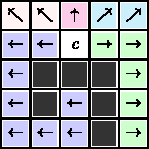
\includegraphics[width=\linewidth]{images/botea-cpd.pdf}
				\caption{Movement-grid for cell $c$\cite{botea-cpd-2013}.}
			\end{wrapfigure}
		
			A \term{compressed path database} (\term*{CPD}) itself is not directly a routing algorithm but rather a technique to efficiently store shortest paths between any two locations\cite{botea-cpd-2013}.
			In other words, the solution of the all-pair shortest paths problem from \Cref{subsubsec:all-pair-shortest-path} can be stored in a CPD without having extensive memory requirements.
			
			The simplest form of a CPD works on a grid rather than a graph, where the number of neighbors is limited and visualization, calculations and compression is simpler.
			For a grid of $n$ cells, $n$ many such grid exist in the CPD, each belongs to a cell $c$ and stores the information on how to get from $c$ to all other cells in the grid.
			Therefore, a potential target cell $t$ contains a movement operation, e.g. \enquote{move to the left cell}, which is the next operation that needs to be performed in order to get from $c$ to $t$ on the shortest path.
			After performing this movement an getting from $c$ to $c'$, the next movement operation to $t$ is stored in the movement-grid of $c'$.
			These steps are performed until $t$ has been reached.
			Answering shortest path queries is therefore linear in the amount of vertices or cells.
			
			The construction of a CPD\cite{botea-cpd-2013} is similarly simple.
			After solving the all-pairs shortest path problem, the result needs to be compressed.
			Uncompressed data is usually too large as the space requirement is in $\bigo{n^2}$ or even $\bigo{n^2 \log n}$ for graphs.
			A combination of compression techniques can be used to get sufficient results.
			This includes the encoding of whole areas with same movement operations, run-length encoding (RLE) and use of default values to reduce the number of explicitly stored values\cite{botea-cpd-2013}.
			Using these techniques, a compression factor of over 950 compared to an uncompressed database can be achieved.
	
\section{Geometric routing}
\label{sec:geometric-routing}

	Finding paths in a geometric domain, also called the \term{euclidean shortest path} problem, is the process of determining shortest paths through open spaces by avoiding obstacles.
	This routing technique takes place under the absence of roads and ways, therefore attributes on these edges, for example surface conditions, are of no use.
	There are two main strategies for finding shortest paths:
	Generating edges through open spaces for graph-based routing or generating a shortest paths map, a structure similar to CPDs.
	
	\subsection{Visibility graphs}
	\label{subsec:visibility-graph}
	
		The first mechanism generates edges and then uses a normal graph-based routing algorithm to actually find the shortest path.
		There are multiple ways on how to create such edges.
		One approach is the creation of a so-called \term{visibility graph}, which is a normal graph with edges between vertices that are visible to each other.
		Or in other words, for any two $u, v \in V$ there is an edge $(u, v) \in E$ if and only if there is no obstacle intersecting this edge.
		A visibility graph might become very large, in fact, the worst-case regarding the size is a complete graph with $\bigo{|V|^2}$ many edges.
		
		Alternatives to the visibility graph generation are based on Voronoi diagrams or skeletonization methods.
		However, routing results on such graphs are not necessarily optimal, since a straight edge between visible vertices is the shortest possible connection.
		These alternative generation approaches do not always create such direct edges\cite{graser-osm-open-spaces}, which leads to detours and longer paths.
		Even though start and destination locations must still be part of the graph to be reachable by routing algorithms, additional edges from and to these locations can be generated with the same algorithm used to create the graph.
	
	\subsection{Continuous Dijkstra}
	\label{subsec:continuous-dijkstra}
	
		The second strategy creates a map of regions starting from a source vertex $s$.
		Each region of this map stores the predecessor vertex, which can be used to determine shortest paths by following the predecessor relations from any given location back to $s$.

		This map can also be seen as a tree with $s$ as its root and each region as a leaf.
		Such a tree might remind one of Dijkstra's algorithm, which creates such a shortest path tree as well to solve the \hyperref[subsubsec:single-source-shortest-path]{single-source shortest path problem}.
		Due to this similarity, this strategy is also called the \term{continuous Dijkstra} paradigm\cite{mitchell-discrete-geodesic}.
		
		To precisely determine these regions, one popular approach is to create \term[wavefront]{wavefronts} propagating through open spaces.
		A well-fitting analogy for this approach is the propagation of sound or water waves traveling through space, folding around obstacles and finally reaching the destination location.
		Recursively following each wave back to its origin yields the shortest path from the source to the destination.
		These wavefronts are also called \term[wavelet]{wavelets}), because they only cover a certain angular range due to collisions and the presence of obstacles.
		
		Each wavefront can collide with edges and vertices but also with other wavefronts.
		After detecting such a collision, the angular region of the wavefront is adjusted depending on the type of collision.
		For each region the origin of the wavefront is known, which enables the query routine to follow these predecessors back to the source.
		The key difficulty of this approach is the efficient propagation of these wavefronts, which means the fast detection of collisions with obstacles and other wavefronts\cite{hershberger-suri}.

\section{Agent-based systems and simulations}

	Simulating complex systems with numerous autonomous individuals, called \term[agent]{agents}, is a complex task.
	Agent-based models help to break down this complexity by simulating each agent separately with its own behavior and decision-making\cite{macal-introductory-tutorial}.
	Interactions between agents and the environment as well as agents with other agents are an essential part of agent-based simulations.
	Each interaction can affect other agents and the environment.
	
	The modeling of agents can be arbitrarily complex.
	Basic agents can interact with other agents and the environment.
	They are able to make decisions on their own, meaning they are autonomous since there is no controlling unit commanding them how to act.
	More complex agents may have a specific goal, are able to adapt themselves to their environment and thus must be able to memorize and plan things.
	
	An agent might be a simulated person but could also be a company, car or other non-living part of the simulated world.
	Many simulations use pedestrians (or generally humans) as agents to better understand human behavior but many more scenarios with other types of agents can be simulated as well\cite{macal-introductory-tutorial}.

	Studying the behavior of pedestrians requires a spatial environment where agents can move and interact with each other.
	Since uncontrolled movement is rather uninteresting, most of the time, algorithms finding optimal paths are involved\cite{kneidl-borrmann-hartmann-navigation,gloor-hybrid-pedestrian-routing,teknomo-millonig-routing}.
	This not only includes \hyperref[sec:graph-routing]{graph-based routing} but often utilizes \hyperref[sec:geometric-routing]{geometric routing} as well\cite{kneidl-borrmann-hartmann-navigation}.
	
	\subsection{The MARS framework}
	
		The algorithm presented in this work was implemented to enhance agent-based simulations created using the framework MARS (Multi-Agent Research and Simulation).
		MARS is a C\#/.NET framework developed by the MARS group, an academic research group of the Hamburg University of Applied Sciences (HAW) in Hamburg, Germany, to create and execute agent-based simulations\cite{mars}.
		The framework offers the necessary components, algorithms and tools to create tick-based simulations consisting of multiple agents, different layers of data and numerous static entities populating the environment.
		
		The MARS framework contains several data structures and algorithms for spatial data and especially for path finding.
		This includes a class representing spatial graphs as well as the A* algorithm, which can determine shortest paths on such graphs.
		MARS also contains numerous spatial indices, mathematical operations and I/O classes, for example to serialize the trajectories of agents.
		 
		This work is based on the MARS framework to be directly usable by simulations, which is why, among other parts, the spatial graph and A* algorithm of MARS are used.
		More details on the design and implementation are given in \Cref{chap:design} and \ref{chap:implementation}.